\graphicspath{{./PBL/images}}

\chapter{Udział w projekcie PBL}

Uczenie poprzez realizację projektów (ang. \angver{Project Based Learning}, PBL) jest metodą przyswajania wiedzy oraz nabywania kompetencji przez studentów poprzez rozwiązywanie rzeczywistych problemów. Dzięki takiemu podejściu, nowe informacje są zapamiętywane na zasadzie ich implementacji w rzeczywistości oraz daje to okazję do aplikacji już wcześniej zdobytej wiedzy i umiejętności. Pozwala to na głębsze zrozumienie treści oraz rozwój innych umiejętności takich jak krytyczne myślenie, praca w grupie i umiejętności komunikacyjne \cite{bib:PBL}. Rozdział ten poświęcony jest takiemu projektowi, w którym brałem udział dwa lata temu. Jego tematyką było zaprojektowanie układu laboratoryjnego przeznaczonego do badań nad wzrostem struktur biologicznych w warunkach mikrograwitacji z wyłączeniem ziemskiego pola magnetycznego. Moje subiektywne odczucia odnośnie tej metody nauki są bardzo pozytywne. Jestem pewien iż dzięki temu projektowi nauczyłem się znacznie więcej niż w przypadku konwencjonalnych metod nauczania. Nabyłem wiele umiejętności praktycznych np. metody tworzenia symulacji opartych o obliczenia równoległe, projektowanie elementów mechanicznych, tworzenie zapotrzebowań na części i surowce oraz wiele innych, które przydały się później w osobistych projektach, praktykach czy też pracy zawodowej.

\section{Cel projektu} \label{cel_projektu}

Celem wspomnianego projektu było zaprojektowanie układu laboratoryjnego, składającego się z
 klatki Helmholtza oraz umieszczonego wewnątrz klinostatu trójwymiarowego. Docelowo taki układ
  pozwalałby na przeprowadzanie badań nad rozwojem roślin w warunkach symulowanej
   mikrograwitacji bez ziemskiego pola magnetycznego. Klatka Helmholtza jest złożeniem trzech
    par cewek Helmholtza w takiej konfiguracji aby osie magnetyczne każdej z par było
     prostopadłe do pozostałych. Pozwala to wytworzyć wektor indukjcji magnetycznej o dowolnym
      kierunku przestrzennym i bardzo wysokiej jednorodności. Wizualizację wyników z przeprowadzonych symulacji można zobaczyć na Rys. \ref{fig:polemag} . Wysoka jednorodność jest kluczowa
       aby generowany wektor indukcji magnetycznej był stały w objętości przeprowadzanego
        eksperymentu. W związku z wymaganiami projektu, wewnętrzna konstrukcja klinostatu
         musiała zostać wykonana tak, aby mieć jak najmniejszy wpływ na panujące wewnątrz
          warunki magnetyczne. Naturalnie rodzi to zagadnienie wyboru materiałów konstrukcyjnych
           klinostatu, które nie powinny mieć właściwości ferromagnetycznych, powinny mieć
            względnie niską przewodność elektryczną w celu eliminacji indukowanych prądów
             wirowych oraz dodatkowym ich atutem będzie niska podatność magnetyczna. Oprócz
              właściwości magnetycznych materiałów istnotne są też możliwości ich obróbki
               termicznej oraz mechanicznej, a również ich forma, co później ma wpływ na
                prostotę montażu urządzenia. Oprócz samych wymagań materiałowych oraz
                 konstrukcyjnych, należało również zapewnić optymalne warunki wzrostowe obiektów
                  badawczych, należało określić odpowiedni rozmiar cewek, aby objętość o wysokim
                   stopniu jednorodności magnetycznej była odpowiednio duża oraz wiele innych.
                    Taki szereg wymagań stworzył bardzo ciekawe i multidyscyplinarne wyzwanie
                     inżynieryjne, które wymagało użycia oraz w niektórych przypadkach
                      stworzenia wielu środowisk symulacyjnych w celu jego rozwiązania. Projekt
                       wykonywany był w zespole 5-cio osobowym na przestrzeni jednego semestru.
                        Powstały na rzecz projektu model komputerowy układu klinostatu wraz z
                         klatką Helmholtza przedstawiony został na Rys.
                          \ref{fig:klatka_helmholtza}.
                          
                                
  \begin{figure}[t]
         	\centering
         	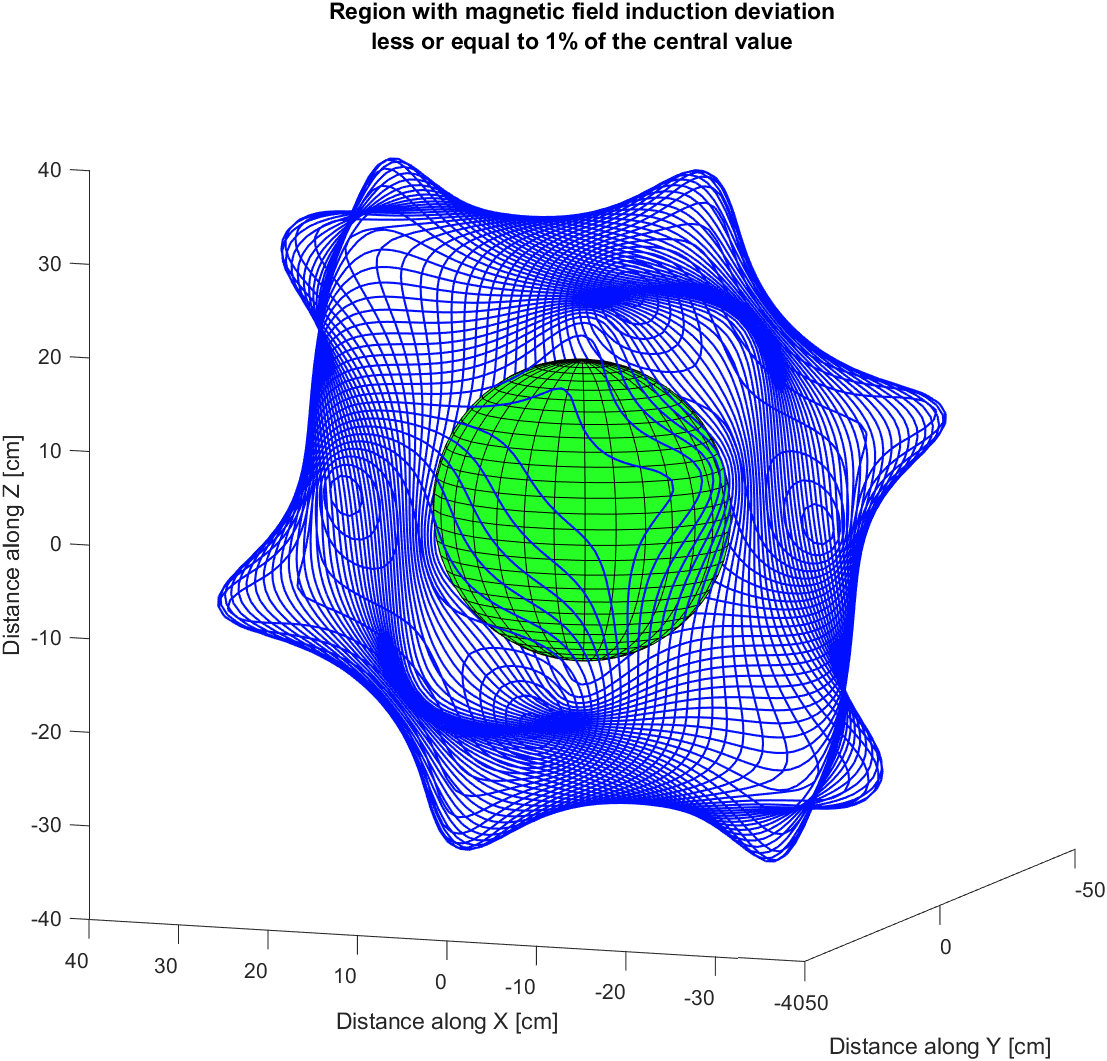
\includegraphics[scale=0.22]{pole_mag}
         	\caption{Wizualizacja objętości w której spełniony jest założony warunek jednorodności pola magnetycznego. Maksymalny odchyłek spełniający założenie przyjęto za 1\% wartości centralnej. Zielona sfera reprezentuje komorę środowiskową wybraną na jej podstawie. Źródło: [opracowanie własne].} 
         	\label{fig:polemag}
  \end{figure}
  

\begin{figure}
	\centering
	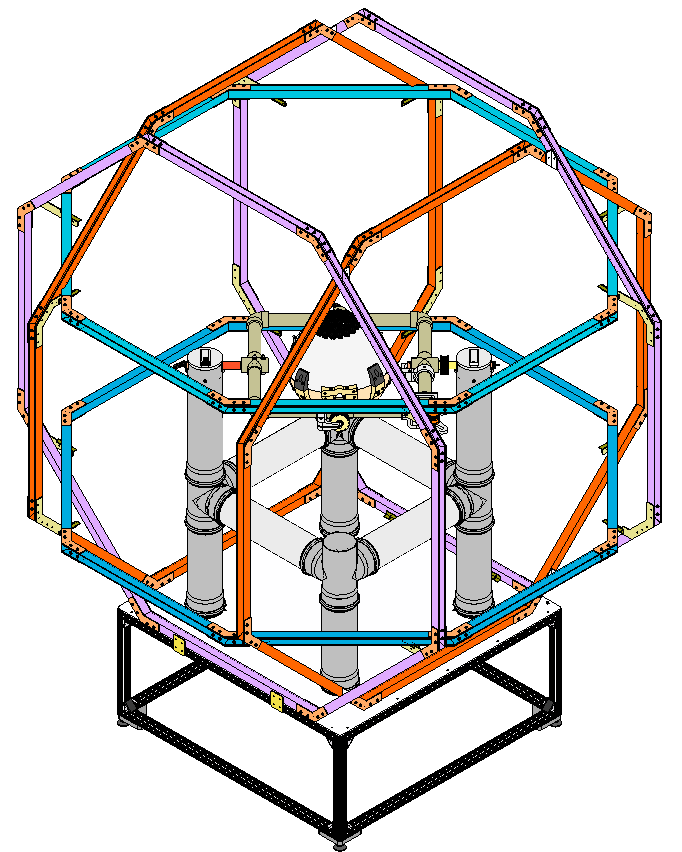
\includegraphics[scale=0.3]{klinostat_klatka}
	\caption{Projekt klatki Helmholtza z klinostatem. Źródło: [opracowanie własne]} 
	\label{fig:klatka_helmholtza}
\end{figure}

\section{Konstrukcja klinostatu} \label{konstrukcja}

Ten podrozdział poświęcony został krótkiemu opisowi konstrukcji samego klinostatu
zaprojektowanego w ramach PBL. Zaprojektowane urządzenie jest klinostatem o dwóch stopniach
swobody, każdy stopień posiada swój osobny napęd. Oznacza to iż jest to maszyna RPM, natomiast
jest możliwość uruchomienia go w trybach klinostatu 2-D oraz 3-D jak opisano w podrozdziale
\ref{klinostat3d}. Zewnętrzna rama klinostatu wykonana została z rur polipropylenowych (PP)
stabilizowanych włóknem szklanym. Odcinki rur wraz z kształtkami 90$^\circ$ oraz
czwórnikami zostały połączone metodą polifuzji termicznej (zgrzewanie). Tego typu rury
wykorzystywane są w instalacjach centralnego ogrzewania, dzięki czemu ich koszt jest
niski. Konstrukcję ramy przedstawiono na Rys. \ref{fig:rama_klinostatu}.Przeprowadzone
analizy elementów skończonych (FEM), wskazały iż materiał ten posiada wystarczającą
wytrzymałość aby wykorzystać go jako element strukturalny ramy klinostatu. Jako wał
obrotowy wykorzystano rurę aluminiową o średnicy \SI{12}{mm}. Wykorzystanie
konwencjonalnych łożysk kulowych w konstrukcji klinostatu nie było wskazane ze
względu na wymagania opisane w podrozdziale \ref{cel_projektu}. Z tego powodu każdy
z interfejsów obrotowych stanowią tuleje ślizgowe wykonane z materiału
iglidur$\copyright$, zaprojektowanego przez firmę IGUS. Większość pozostałych
elementów została wykonana w technologii druku przestrzennego z materiału PETG.
Konstrukcję jednego z czterech czwórników ramy przedstawiono na Rys.
\ref{fig:czwórnik}. Wewnętrzny stopień swobody składa się z kulistej komory
środowiskowej, która posiada swój dedykowany komputer o niskiej mocy,
monitorujący panujące wewnątrz warunki, oraz sterujący oświetleniem.
Zasilanie do wnętrza komory doprowadzone jest przez szereg złącz
ślizgowych, a przewody poprowadzone są wewnątrz ramy klinostatu. Podobne
rozwiązanie wykorzystano w obwodzie doprowadzjącym wodę, przewody
prowadzone są wewnątrz ramy klinostatu, a przy elementach obrotowych
zastosowano kolanka obrotowe. Rozmiar komory oraz typ i moc oświetlenia
zostały wyznaczone na podstawie wyników symulacji stworzonych na rzecz
projektu. Jej projekt przedstawiony został na Rys. \ref{fig:komora}.
Mocowania śrubowe zostały w większości zrealizowane za pomocą śrub
poliamidowych (PA). Komora została zaprojektowana tak, aby umożliwić operatorowi dostęp do jej
wnętrza bez konieczności jej demontażu z ramy klinostatu.

\begin{figure}[]
	\centering
	
	\begin{subfigure}[b]{.49\textwidth}
		\centering
		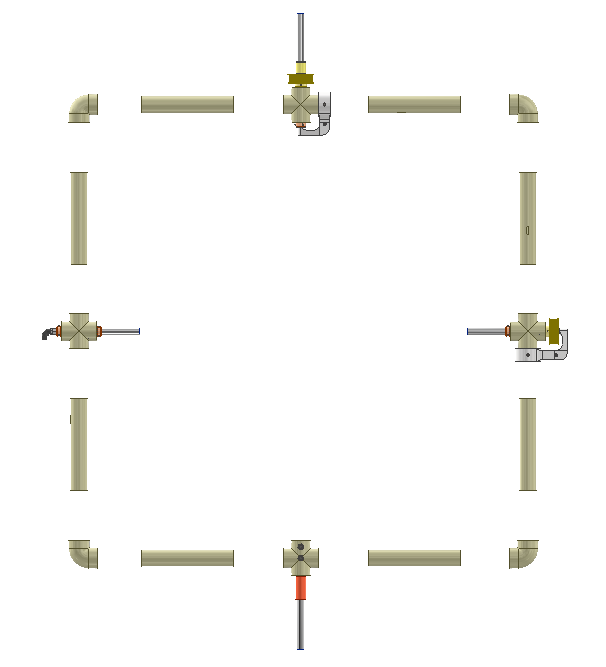
\includegraphics[width=\textwidth]{rama_40_aisass}
		\caption{Rama klinostatu} 
		\label{fig:rama_klinostatu}
	\end{subfigure}
	\hfill%
	\begin{subfigure}[b]{.49\textwidth}
		\centering
		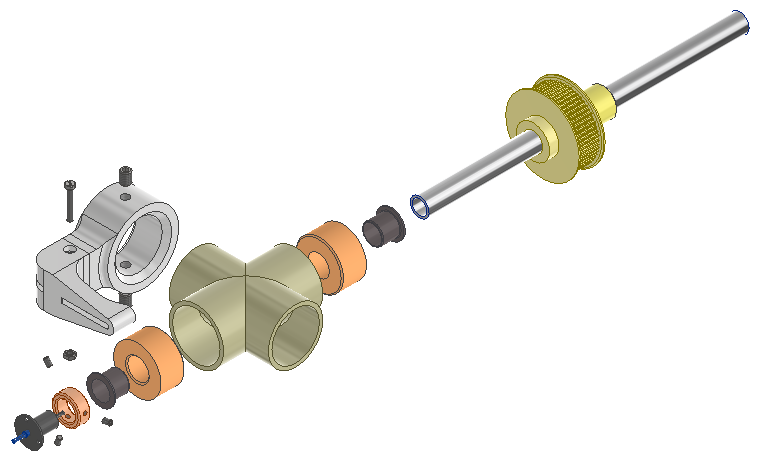
\includegraphics[width=\textwidth]{2_diss}
		\caption{Czwórnik ramy klinostatu.} 
		
		\label{fig:czwórnik}
	\end{subfigure}\vspace{15mm}%
	
	\begin{subfigure}{.8\textwidth}
		\centering
		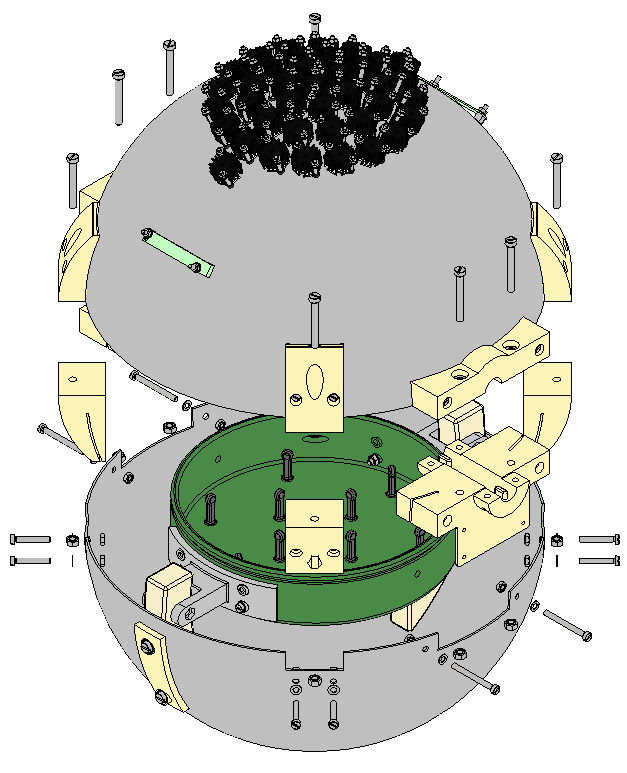
\includegraphics[scale=0.3]{Komora_tweaked_colors_exploded}
		\caption{Komora środowiskowa.} 
		\label{fig:komora}
	\end{subfigure}
	
	\caption{Przykładowe części modelu komputerowego projektu. Źródło: [opracowanie własne]}
	
\end{figure}


\section{Modyfikacje projektu}

Z uwagi na dużą złożoność realizowanego projektu, zakończył się on na etapie ukończonego modelu komputerowego. Konstrukcję całego urządzenia rozpoczęto rok po
   zakończeniu się projektu PBL w zespole dwuosobowym, w którego skład wchodziłem. Podczas
    konstrukcji napotkano wiele problemów, które nie zostały przewidziane na etapie prac
     projektowych i wymagały stworzenia nowych elementów urządzenia, bądź zmodyfikowania już
      istniejących komponentów. Oprócz tego wymagane było również stworzenie metod
       konstrukcyjnych tak aby zachować jego kluczowe cechy, oraz aby mogło ono zostać wykonane
        bez użycia kosztownych metod obróbki takich jak wspomagana numerycznie obróbka maszynowa
         (ang. \angver{Computerized Numerical Control}, CNC). Takich poprawek stworzono bardzo
          wiele na drodze konstrukcji urządzenia, natomiast w tym podrozdziale zostaną opisane
           dwie najbardziej kluczowe dla jego poprawnego działania.
           

\subsection{Przeciwwaga ramy klinostatu}

Podczas pierwszych prób uruchomieniowych klinostatu napotkano okresowo pojawiający się moment
 siły, który hamował ruch obrotowy urządzenia przez zbyt duże obciążenie układu napędowego. Za
  jedno ze źródeł tego problemu zidentyfikowano asymetrię obciążenia ramy klinostatu, powodowaną
   układem zmiany kierunku pasa układu napędowego komory środowiskowej, który ulokowany jest na
    rogu ramy. W tym celu na przeciwległym rogu zamontowano przeciwwagę, które generowała moment
     siły o tym samym kierunku, natomiast o przeciwnym zwrocie. Przeciwwaga składa się z
      drukowanego uchwytu oraz kawałka rury PP, która wypełniona jest piaskiem w celu
       zapewnienia odpowiedniej masy. Skonstruowana oraz zamontowana przeciwwaga przedstawiona
        została na Rys. \ref{fig:przeciwwaga}.

\begin{figure}[H]
	\centering
	\setlength{\fboxsep}{0pt}
	\setlength{\fboxrule}{1pt}
	\fbox{\includegraphics[scale=0.045]{przeciwwaga}}
	\caption{Zamontowana przeciwwaga. Źródło: [opracowanie własne].} 
	\label{fig:przeciwwaga}
\end{figure}

\subsection{Przekładnie walcowe}

Drugą bardzo istotną dla działania klinostatu modfikacją, był projekt i konstrukcja dwóch
 przekładni walcowych, które zwiększają dostępny moment obrotowy układu napędowego. Z uwagi na
  to iż klinostat przeznaczony będzie przedewszystkim do badań nad organizmami roślinnymi, jego
   prędkość obrotowa powinna mieścić się w zakresie od 1 do 2 RPM. W pierwotnej konfiguracji
    klinostat był w stanie osiągnąć znacznie większe prędkości obrotowe, co umożliwiło
     zastosowanie wspomnianych przekładni. Zaprojektowanie przekładnie stosują redukcję obrotów
      silników 4:1. Pozwala to osiągnąć czterokrotnie wyższy moment obrotowy przed głównym kołem
       napędowym klinostatu. Model przekładni widoczny jest na Rys. \ref{fig:projekt
       	 przekładni}. Przekładnia składa się z dwóch kół zębatych o liczbie zębów odpowiednio 12 i 48. Duże koło zębate jest
          łożyskowane w dwóch miejscach przez konwencjonalne łożyska kulowe, ze względu na to iż przekładnie znajdują się w wystarczająco dużej odległości od objętości jednorodnego
            pola magnetycznego. Na małym kole zębatym umieszczono dodatkowo wpusty umożliwiajace
             montaż enkoderów, jeśli zajdzie taka potrzeba. Całość zamknięta została w korpusie
              odpowiedzialnym za ochronę kół przez pyłem oraz zapobiegającym wydostaniu się
               smaru na zewnątrz. Skonstruowana przekładnia z nałożonym kołem pasowym
                przedstawiona jest na Rys. \ref{fig:gotowa przekładnia}. Zastosowanie przekładni
                 znacznie poprawiło działanie klinostatu, przy jednoczesnym zachowaniu wymaganej
                  prędkości obrotowej urządzenia.       


\begin{figure}
	\centering
	
	\begin{subfigure}[h]{.49\textwidth}
		\centering
		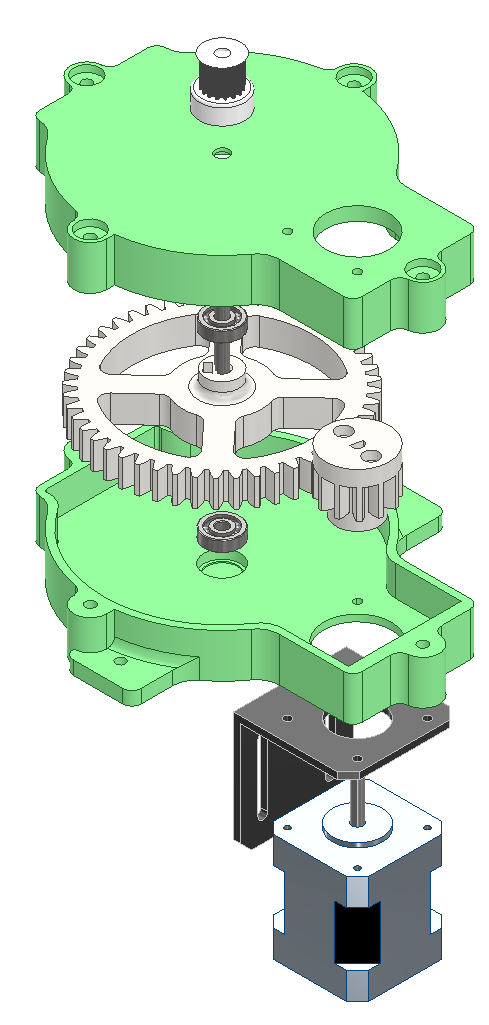
\includegraphics[width=.4\textwidth]{przekladnia_projekt_exploded_shaded}
		\caption{Projekt przekładni} 
		\label{fig:projekt przekładni}
	\end{subfigure}
	\hfill%
	\begin{subfigure}[h]{.49\textwidth}
		\centering
		\setlength{\fboxsep}{0pt}
		\setlength{\fboxrule}{1pt}
		\fbox{\includegraphics[width=.8\textwidth, angle=-90]{przekladnia_gotowa}}
		\caption{Skonstruowana przekładnia.} 
		\label{fig:gotowa przekładnia}
	\end{subfigure}

	\caption{Przekładnie klinostatu. Źródło: [opracowanie własne]}
	
\end{figure}

\section{Komora środowiskowa}

Wewnętrzny stopień swobody klinostatu składa się z kulistej komory środowiskowej. Jej celem jest zapewnienie odpowiedniego podłoża do wzrostu badanej struktury, oraz dopilnowanie optymalnych warunków wzrostowych poprzez dostarczanie wody ze składnikami odżywczymi oraz odpowiednie oświetlenie. Konieczne jest odizolowanie obiektu eksperymentu od zewnętrznych źródeł światła, aby zapewnić kontrolowane oraz powtarzalne warunki przeprowadzania eksperymentu. Komora wykonana została z globusa o średnicy \SI{320}{mm} poddanego specjalnej obróbce mechanicznej. Półsfery zostały odseparowane wzdłuż zgrzewu przy pomocy tokarki, a następnie każda z nich została poddana odpowiedniej obróbce. Model półsfer komory przedstawiono na Rys. \ref{fig:globus}. Na zawętrznej części komory wyznaczono miejsca przeznaczone do montażu kamer oraz oświetlenia. Półsfery łączone są za pomocą specjalnych, drukowanych łączników, które nasuwają się na przygotowane wcięcia i łączone są przez połączenia śrubowe (Rys. \ref{fig:łącznik_globus}). Analogicznie rozwiązanie zostało połączenie komory z wałem obrotowym. W środku komory zamontowany jest kosz uprawny, którego wysokość może być regulowana w zależności od spodziewanej wysokości struktury wzrostowej. W koszu zamontowane są specjalne elementy mocowania przewodu doprowadzającego wodę, które również wyznaczają jego spiralny tor. Wewnątrz komory rozmieszczony jest szereg czujników monitorujących warunki wzrostowe oraz jej orientację względem wektora grawitacji w czasie. Na komorze zamontowany jest również komputer niskiej mocy, odpowiedzialny za zbieranie danych z czujników i przesyłanie ich do głównej jednostki kontroli poprzez sygnał bezprzewodowy.

\begin{figure}
	\centering
	
	\begin{subfigure}[b]{.49\textwidth}
			\centering
			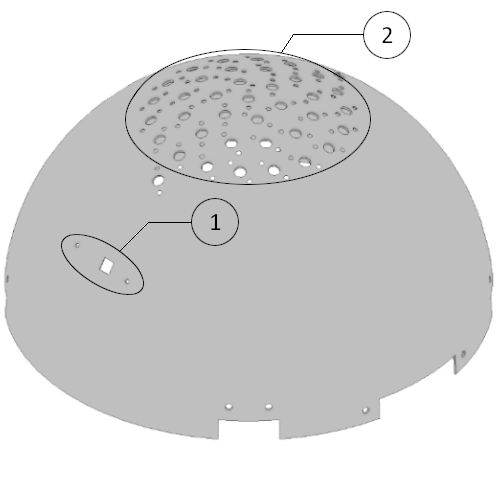
\includegraphics[width=.6\textwidth]{top_half_marked}
			\caption{Półsfera górna.} 
			\label{fig:globus_top}
	\end{subfigure}
	\hfill%
	\begin{subfigure}[b]{.49\textwidth}
			\centering
			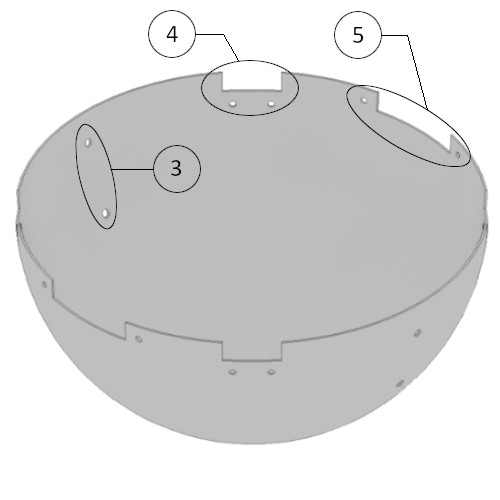
\includegraphics[width=.6\textwidth]{bot_half_marked}
			\caption{Półsfera dolna.} 
			\label{fig:globus_bot}
	\end{subfigure}
	\caption{Spreparowane półsfery z oznaczonymi elementami. \textbf{1} - otwory montażu kamery, \textbf{2} - otwory montażu oświetlenia, \textbf{3} - otwory montażu koszyka, \textbf{4} - wcięcia oraz otwory montażu łącznika półsfer, \textbf{5} - wcięcia oraz otwory montażu półsfery z wałem obrotowym. Źródło: [opracowanie własne]}
	\label{fig:globus}

\end{figure}

\begin{figure}
	
	\centering
	\includegraphics[scale=.25]{bottom_half_connector_framed}
	\caption{Łącznik montowany na półsferze komory. Źródło: [opracowanie własne]} 
	\label{fig:łącznik_globus}
	
\end{figure}

\section{Kontrola klinostatu}

Jak wspomniano w podrozdziale \ref{konstrukcja}, oba stopnie swobody klinostatu mają swoją niezależną jednostkę napędową. Jako źródło ruchu obrotowego wybrano silniki krokowe w standardzie NEMA 17, model 42BYGHM809. Są to silniki o rozdzielczości ruchu 400 kroków na pełen obrót, oraz momencie obrotowym wynoszącym \SI{0,48}{Nm}. Podłączone są one do opisanych wcześniej przekładni walcowych, których wyjścia zakończone są kołami pasowymi. Ruch obrotowy jest następnie przenoszony przez pasy zębate, które ostatecznie łączą się z głównymi kołami napędowymi klinostatu na szczycie konstrukcji jego podstawy. Na silniki krokowe zdecydowano się ze względu na prostotę ich sterowania oraz możliwość dokładnego pozycjonowania w razie potrzeby rozszerzenia urządzenia o taką funkcjonalność. Silniki podłączone są bezpośrednio do obudowy zawierającej elektronikę sterującą klinostatem. Elektronika sterująca składa się z platformy Arduino Leonardo stanowiącej sterownik układu, nakładki RAMPS dla platform Arduino, dwóch sterowników silników krokowych A4988, konwertera UART/USB w celu komunikacji z komputerem przez interfejs USB oraz przetwornicy step-up, konwertującej napięcie zasilacza 12V do 36V dla zasilania silników. W obudowie zamontowany został również wentylator chłodzący sterowniki silników. Zmontowany układ przedstawiony został na Rys. \ref{fig:elektronika}. 

\begin{figure}[ht]
	\centering
	\setlength{\fboxsep}{0pt}
	\setlength{\fboxrule}{1pt}
	\fbox{\includegraphics[width=.6\textwidth]{elektronika}}
	\caption{Elektronika klinostatu. Źródło: [opracowanie własne]} 
	\label{fig:elektronika}
\end{figure}